\documentclass[tikz]{standalone}
\usepackage{xcolor}
\begin{document}
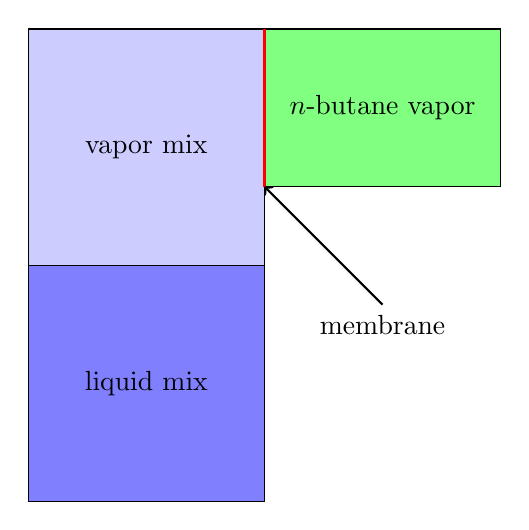
\begin{tikzpicture}
    \draw[fill=blue!50] (0,0) rectangle (3,3) node[midway]{liquid mix};

    \draw[fill=blue!20] (0,3) rectangle (3,6) node[midway]{vapor mix};

    \draw[fill=green!50] (3,6) rectangle (6,4) node[midway]{$n$-butane vapor};
    
    \draw[line width=1pt, red] (3,6) -- (3,4);
    
    \draw[->, black, thick] (4.5,2.5) node[anchor=north]{membrane} -- (3,4);
\end{tikzpicture}
\end{document}